\documentclass[12pt]{beamer}

\usepackage{amsmath,amssymb}
\usepackage{algpseudocode}
\usepackage{algorithm}
\usepackage{caption, subcaption}
\usepackage{graphicx}
\usepackage{hyperref}
\graphicspath{{img/}}
\DeclareGraphicsExtensions{.png}

%custom commands for math ease
\renewcommand{\d}[1]{\dot{#1}}
\newcommand{\fn}[1]{\footnote{\footnotesize #1}}
\newcommand{\grad}{\nabla}
\newcommand{\mat}[4]{\begin{bmatrix} #1 & #2\\#3 & #4\end{bmatrix}}
\newcommand{\e}{\varepsilon}
\newcommand{\pic}[1]{\includegraphics[clip = true, trim=0cm 0cm 4cm 0cm, width = 5cm, height = 3.8cm, keepaspectratio = true]{#1}}

%page layout stuff
\usetheme{Frankfurt}
\usecolortheme{beetle}
%\usepackage{remreset}% tiny package containing just the \@removefromreset command
%\makeatletter
%\@removefromreset{subsection}{section}
%\makeatother
%\setcounter{subsection}{1}
\setbeamersize{text margin left=.2cm,text margin right=.2cm}

%title info
\title[]
{
  Automatic Differentiation Applied \\
  to QR Iteration
}
\author{Peter Solfest}
\institute{University of Minnesota\\Department of Computer Science and Engineering}
\date{Research Group Meeting 11/11/2014}

\begin{document}

	%title
	\frame{\titlepage}

	%table of contents
	\begin{frame}
		\frametitle{Outline}
		\tableofcontents
	\end{frame}
	

	\section{Automatic Differentiation}
	\begin{frame}{}
    \centering
    {\huge Automatic \\Differentiation \\(AD)}	
	\end{frame}	
	
	\begin{frame}{Big Picture}
    \begin{itemize}
      \item At its core, computer code consists of arithmetic and logical operations
      \item AD applies elementary differentiation rules to the arithmetic operations
    \end{itemize}
    \begin{center}
    Can overload operators to achieve this.
    
    Examples:
    \begin{align*}
      a + b &\to {a+b, \partial a + \partial b}\\
      a \cdot b &\to {a \cdot b, \partial a \cdot b + a \cdot \partial b}\\
      \sin(a) &\to {\sin(a) , \cos(a) \cdot \partial a}\\
      \cdots
    \end{align*}
    \end{center}
	\end{frame}

  \begin{frame}{Forward Mode}
    \begin{itemize}
      \item Calculate effect on output due to perturbed inputs
      \item Input perturbation direction is provided to seed the calculation
      \item Notation: $\d{w}$ is the derivative w.r.t. input perturbation
    \end{itemize}
    
    \begin{figure}[h!]
      \centering
      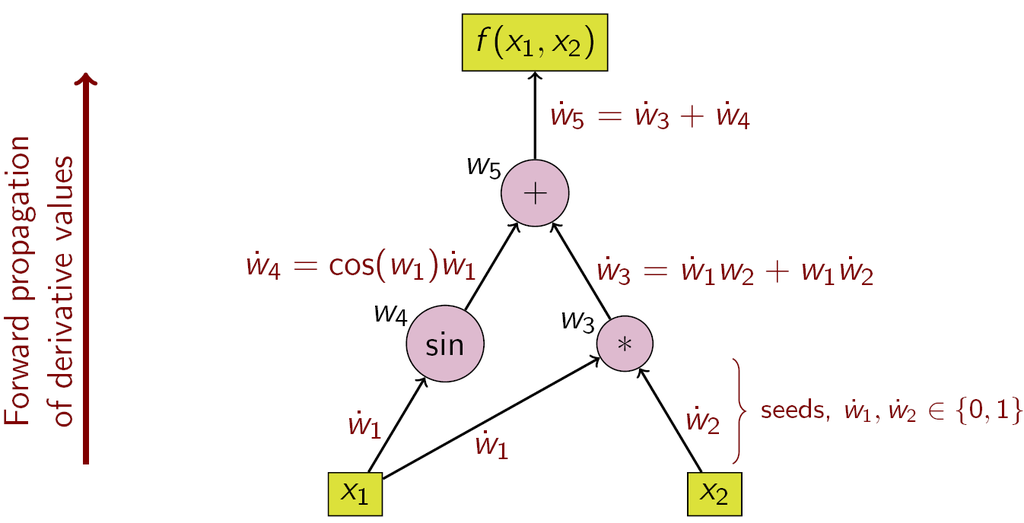
\includegraphics[height=.5\textheight]{forwardMode}
      \caption{The subscripts represent intermediate steps\fn{Figure from wikipedia's \href{http://en.wikipedia.org/wiki/Automatic_differentiation}{Automatic Differentiation} page}}
    \end{figure}

  \end{frame}

  \begin{frame}{Reverse Mode}
    \begin{itemize}
      \item Calculate what input perturbation creates output perturbation
      \item Output perturbation direction is provied to seed the calculation
      \item Notation: $\bar{w}$ is the derivative w.r.t. input perturbation
    \end{itemize}

    \begin{figure}[h!]
      \centering
      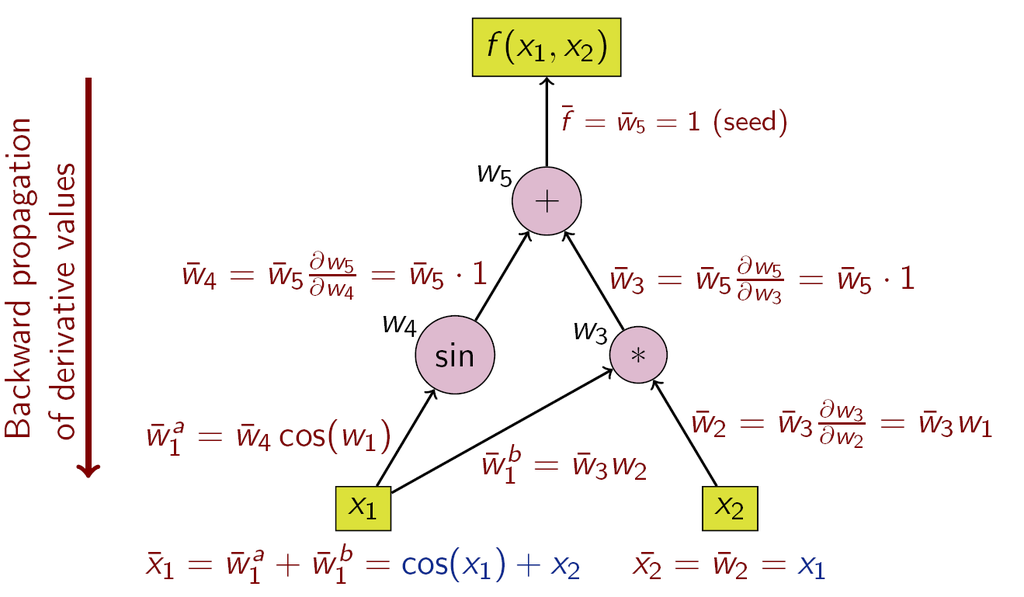
\includegraphics[height=.5\textheight]{reverseMode}
      \caption{The subscripts represent intermediate steps\fn{Figure from wikipedia's \href{http://en.wikipedia.org/wiki/Automatic_differentiation}{Automatic Differentiation} page}}
    \end{figure}
  \end{frame}

  \begin{frame}{Abstract Formulation}
    \begin{itemize}
      \item An algorithm can be viewed as a map
        \[f:\mathbb{R}^m \to \mathbb{R}^n\]
      \item Forward Mode calculates directional derivatives of $f$ (the directions are the seeds)
      \item Reverse Mode calculates the gradient of $f$ (if seeded with 1, otherwise is a scaled gradient)
    \end{itemize}

  \end{frame}

  \begin{frame}{Forwards vs. Backwards}
    \centering
    For an algorithm $\vec{f}:\mathbb{R}^m \to \mathbb{R}^n$\\[.5in]
    \begin{table}[h!]
      \begin{tabular}{l | l}
        Forward Mode & Backwards Mode\\\hline
        simple memory access & complicated memory access\\
        1-2 function evaluations for $\grad \vec{f} \cdot \vec{d}$  & 1-10 function evaluations for $\grad f_i$\\
        $m$ sweeps to compute $\grad \vec{f}$ & $n$ sweeps to compute $\grad \vec{f}$
      \end{tabular}
    \end{table}
    Will focus on forward mode
  \end{frame}

  \begin{frame}{Schur Decomposition AD}
    For $A \in \mathbb{R}^{n \times n}$, the Schur decomposition is
    \begin{align*}
      A &= Q S Q'\\
      Q'Q &= I
    \end{align*}
    with $S$ upper triangular\fn{except 2x2 blocks on diagonal}

    Thus
    \begin{align*}
      \d{A} &= \d{Q}SQ' + Q\d{S}Q' + QS\d{Q}'\\
      Q' \d{A} Q &= P S + S P' + \d{S}\\
      Q' \d{A} Q &= P S - S P + \d{S}
    \end{align*}
    Where $P = Q'\d{Q}$, and the orthonormality of $Q$ yields that $P = -P'$

  \end{frame}

  \begin{frame}{Schur Decomp AD Algorithm}
    \begin{itemize}
      \item Treat $\d{A}$ as the seeded input, define $B = Q' \d{A} Q$
      \item Noting $S, \d{S}$ are upper triangular and $P$ is skew symmetric, note
      \begin{align*}
        \mat{B_{11}}{B_{12}}{B_{21}}{B_{22}} &= \mat{P_{11}}{-P_{21}'}{P_{21}}{P_{22}} \mat{S_{11}}{S_{12}}{0}{S_{22}} - \mat{S_{11}}{S_{12}}{0}{S_{22}} \mat{P_{11}}{-P_{21}'}{P_{21}}{P_{22}}\\
        &+ \mat{\d{S}_{11}}{\d{S}_{12}}{0}{\d{S}_{22}}
      \end{align*}
      \item The $(21)$ block yields $B_{21} = P_{21}S_{11} - S_{22}P_{21} + 0$, use triangular sylvester equation solver\fn{e.g. Octave's \texttt{syl}. Or use the same splitting trick}
      \item Recursively solve the $(11)$ and $(22)$ blocks
      \item Compute $\d{Q} = QP$ and $\d{S} = B - PS + SP$
    \end{itemize}
  \end{frame}

  \begin{frame}{Schur Decomp AD Performance}
    Given a Schur decomposition $A = Q*S*Q'$, and seed $\d{A}$: 
    \[A + \e\d{A} = (Q + \e \d{Q})(S + \e \d{S})(Q + \e \d{Q})' + O(\e^2)\]
    \[ (Q + \e \d{Q})'(Q + \e \d{Q}) = I + O(\e^2)\]
    Following is the difference (error) observed as measured in the Frobenius norm.
    \begin{figure}[h!]
      \centering
      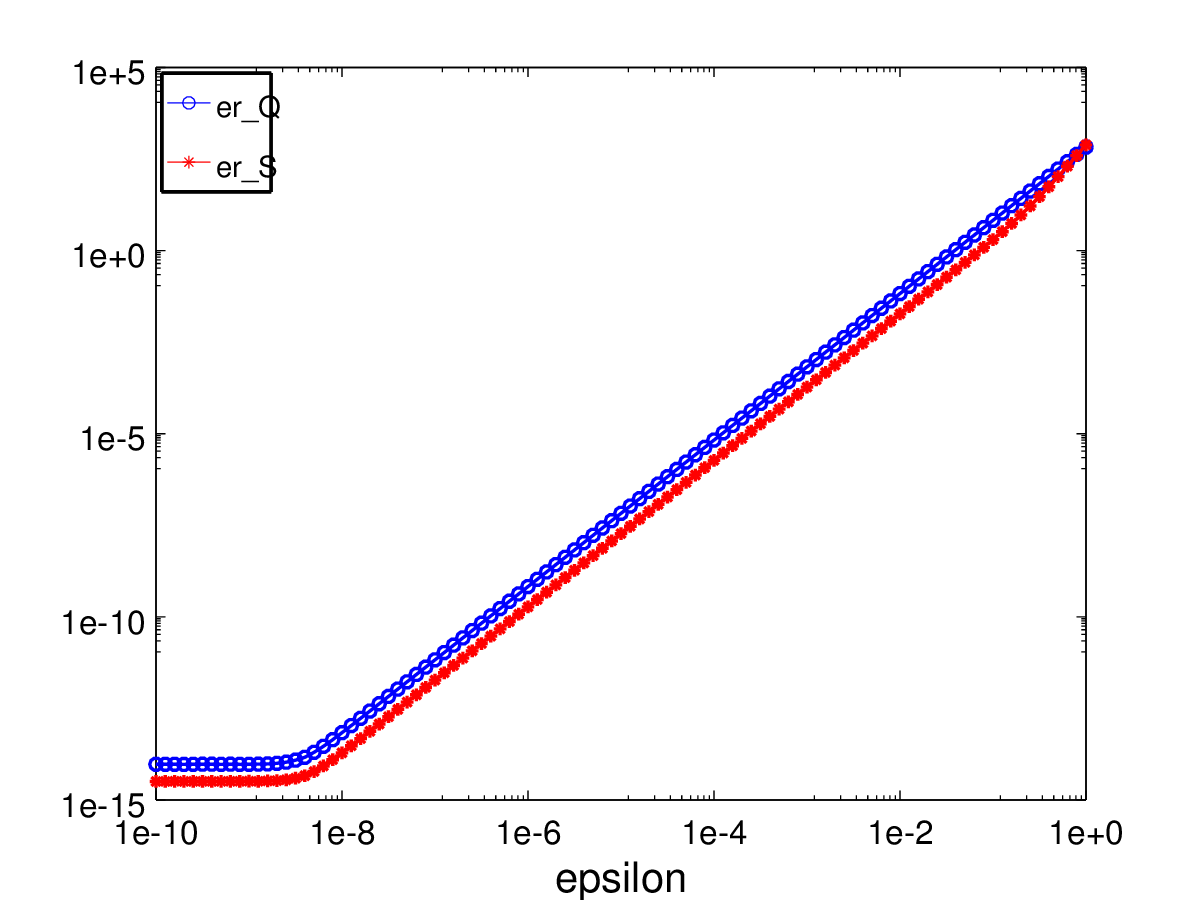
\includegraphics[width = .3\textwidth]{schurErr}
    \end{figure}
    On 10 random matrices in $\mathbb{R}^{400 \times 400}$, octave's built in \texttt{schur} function took 3.78 seconds (cumulative),
    and the schurAd algorithm spent 3.47 seconds (cumulative) calculating the derivatives.
  \end{frame}

	\section{Implicit QR Iteration}
	\begin{frame}{}
	  \centering
    {\huge Implicit multishift QR \\and Enhancements}
	\end{frame}

  \begin{frame}{Multishift QR}
    Multishift QR sweep:
    \begin{algorithmic}
      \Function{MQRSweep}{H,$\vec{\sigma}$}
        \State form householder vector from $1^{st}$ column of $\prod_{i=1}^{s}(H - \sigma_i I)$
        \State Apply householder transformation to $H$ using this vector
        \State Reduce $H$ to hessenberg form
        \State Deflate $H$ if small entry on subdiagonal\\
        \Return $H$, deflated eigenvalues
      \EndFunction
    \end{algorithmic}
    In practice for $s > 5$, add the shifts in $5$ at a time rather than all at once.\cite{}
  \end{frame}

  \begin{frame}{One 'Sweep'}
    \vspace*{-.8cm}
    \begin{figure}[h!]
      \centering
      \begin{minipage}[t]{.5\linewidth}
        \centering
        \pic{simpSweep1}
      \end{minipage}~
      \begin{minipage}[t]{.5\linewidth}
        \centering
        \pic{simpSweep2}
      \end{minipage}

      \begin{minipage}[b]{.5\linewidth}
        \centering
        \pic{simpSweep3}
      \end{minipage}~
      \begin{minipage}[b]{.5\linewidth}
        \centering
        \pic{simpSweep4}
      \end{minipage}%
    \end{figure}
  \end{frame}

  \begin{frame}{QRI AD Performance}
    Consider $f:\mathbb{R}^s \to \mathbb{R}^{n \times n}$, where the inputs
    are the shifts $\vec{\sigma}$, and the output is the matrix after a sweep of QRI.

    Then we have in the direction $\vec{d}$
    \[
      f(\vec{\sigma}) + \e \d{f}(\vec{\sigma}) = f(\vec{\sigma} + \e \vec{d}) + O(\e^2)
    \]
    Below is the difference (error) observed as measured in the Frobenius norm.
    \vspace*{-1cm}
    \begin{figure}[h!]
      \centering
      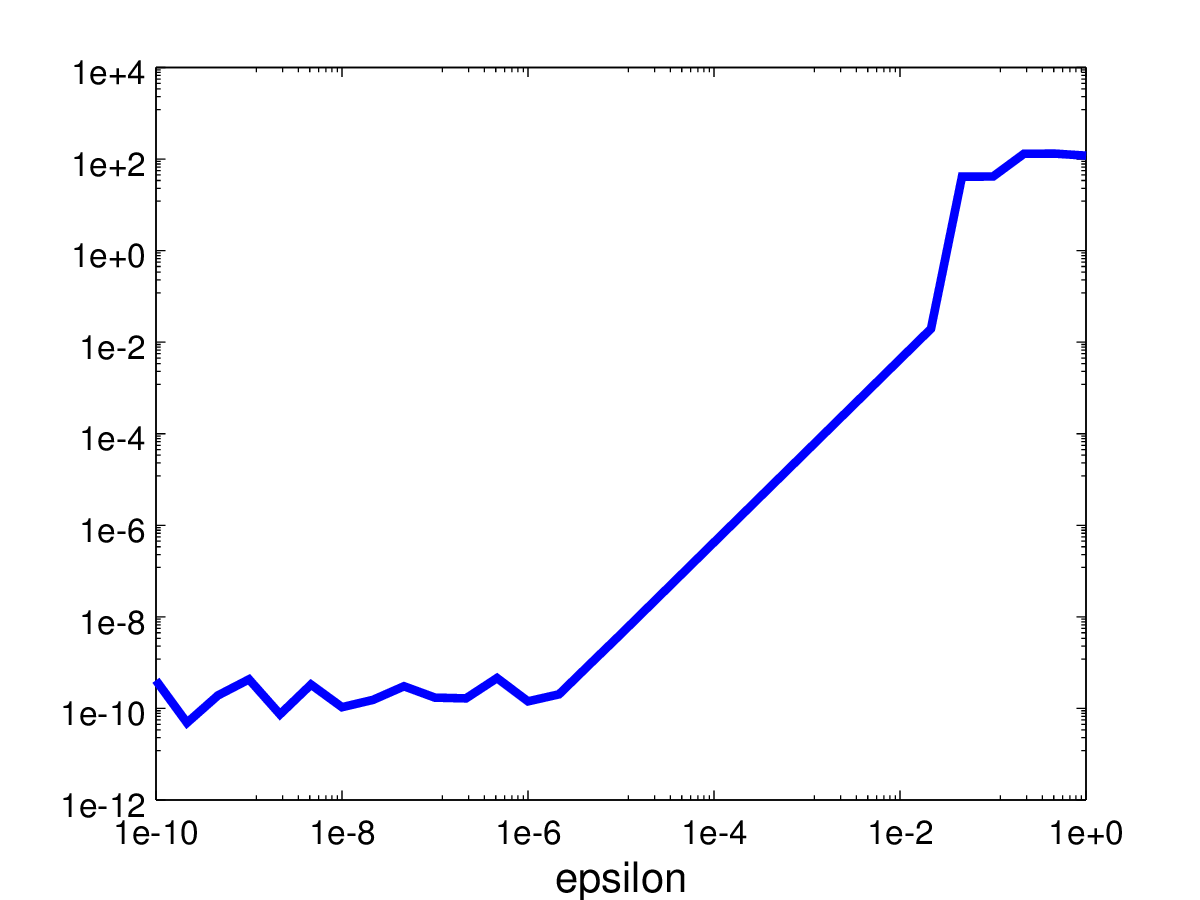
\includegraphics[width = .3\textwidth]{qriErr}
    \end{figure}
    On 10 random matrices in $\mathbb{R}^{400 \times 400}$, using 20 shifts, a QRI sweep took 8.74 seconds (cumulative),
    and with 1 seed it took 22.47 seconds (cumulative).
  \end{frame}

  \begin{frame}{AD Definitions}
    \begin{itemize}
      \item the shifts $\vec{\sigma}$ form a natural set of inputs
      \item $f:\mathbb{R}^s \to \mathbb{R}^t$
      \item define $J_{i,j}(\vec{\sigma}) = \dfrac{\partial f_i}{\partial \sigma_j}(\vec{\sigma})$, so $J \in \mathbb{R}^{t \times s}$
      \item Assume we want to find $\vec{\sigma}$ such that $f(\vec{\sigma}) = \vec{0}$
      \item Newton's method provides an update procedure $\vec{\sigma}^{(n+1)} = \vec{\sigma}^{(n)} - J^{-1}(\vec{\sigma}^{(n)}) f(\vec{\sigma}^{(n)})$
    \end{itemize}
  \end{frame}


  \begin{frame}{AD Variation on standard QRI}
    Standard Algorithm:
    \begin{algorithmic}
      \Repeat
        \State $\sigma \gets eig(H_{n-s:n,n-s:n})$ 
        \State $H \gets MQRSweep(H,\sigma)$ 
      \Until{length(H) $<$ 2}
    \end{algorithmic}

    AD Variation:
    
    Choose the output of $f$ to be the $s$ bottommost subdiagonals

    \begin{algorithmic}
      \State Choose $\sigma$ 
      \Repeat
        \State $\d{H} \gets MQRSweep(H,\sigma)$ for seeded $I_{s \times s}$
        \State Deflate $H$ if possible
        \State Form $J(\vec{\sigma})$
        \State $\vec{\sigma} \gets \vec{\sigma} - J^{-1}(\vec{\sigma}) f(\vec{\sigma})$
      \Until{length(H) $<$ 2}
    \end{algorithmic}

  \end{frame}

  \begin{frame}{Aggresive Early Deflation}
    \begin{itemize}
      \item drive the bulges through the matrix via QRI
      \item perform a Schur decomposition on the bottom portion containing the bulges, introducing a spike
      \item deflate matrix if spike values are below a tolerance
    \end{itemize}

    \begin{figure}[h!]
      \begin{minipage}[t]{.5\linewidth}
        \centering
        \pic{agDef1}
      \end{minipage}~
      \begin{minipage}[t]{.5\linewidth}
        \centering
        \pic{agDef2}
      \end{minipage}
    \end{figure}
    
    For the AD version, the outputs are the bottom $s$ values on the spike.
  \end{frame}

  \begin{frame}{Middle Deflation}
    \begin{enumerate}
      \item Bulges are driven from both ends
      \item When they meet, a Schur decomposition is performed, generating 2 spikes\cite{}
      \item If the tips of the spikes have enough zeros, can split matrix in the middle
    \end{enumerate}

    \begin{itemize}
      \item Performing this in the middle of QRI was proposed in Braman %\cite{}
      \item the outputs for the AD algorithm will be the tips of the spikes
    \end{itemize}
  \end{frame}

  \begin{frame}{One 'Sweep' to middle}
    \vspace*{-.8cm}
    \begin{figure}[h!]
      \centering
      \begin{minipage}[t]{.5\linewidth}
        \centering
        \pic{midDef1}
      \end{minipage}~
      \begin{minipage}[t]{.5\linewidth}
        \centering
        \pic{midDef2}
      \end{minipage}

      \begin{minipage}[b]{.5\linewidth}
        \centering
        \pic{midDef3}
      \end{minipage}~
      \begin{minipage}[b]{.5\linewidth}
        \centering
        \pic{midDef4}
      \end{minipage}%
    \end{figure}
  \end{frame}

  \begin{frame}{Implementation Details}
    \begin{itemize}
      \item Schur decomposion is not unique since the eigenvalues can be reordered.
        Thus they were reordered to yield minimum value in the spike tips \cite{}
      \item For aggressive early deflation, a second spike on the deflated matrix
        without another QR iteration can yield further deflatable eigenvalues which are deflated\cite{}
    \end{itemize}
  \end{frame}

	\begin{frame}{Results}
    \begin{itemize}
      \item Run on matrices generated by normal distribution of random numbers
      \item the Jacobian becomes singular very quickly.
      \item Using a low-rank approximation to the Jacobian, causing shifts to converge when deflation isn't possible
      \item Re-initializing shifts when this happens leads to convergence to another non-deflatable minima
    \end{itemize}
	\end{frame}
	
	\nocite{*}
	\begin{frame}{Bibliography}
		\bibliographystyle{plain}
		\bibliography{biblio}
	\end{frame}
	
\end{document}
